\documentclass{article}
\usepackage[utf8]{inputenc}
\usepackage[english]{babel}
\usepackage[font=small,labelfont=bf]{caption}
\usepackage{geometry}
\usepackage{natbib}
\usepackage{pxfonts}
\usepackage{graphicx}
\usepackage{newfloat}
\usepackage{setspace}
%\doublespacing

\newcommand{\argmax}{\mathop{\mathrm{argmax}}\limits}

\title{\textit{Extended data for}: Towards human Super EEG?}
\author{Lucy L. W. Owen, Andrew C. Heusser, and Jeremy R. Manning\\Department of Psychological and Brain Sciences\\Dartmouth College, Hanover, NH 03755, USA\\Corresponding author: jeremy.r.manning@dartmouth.edu}

\bibliographystyle{apa}

\begin{document}
\maketitle

\setcounter{equation}{0}
\setcounter{figure}{0}
\setcounter{table}{0}
\setcounter{page}{1}
\setcounter{section}{0}
\makeatletter
\renewcommand{\theequation}{S\arabic{equation}}
\renewcommand{\thefigure}{S\arabic{figure}}
\renewcommand{\bibnumfmt}[1]{[S#1]}
\renewcommand{\citenumfont}[1]{S#1}


\section*{Overview}
This document provides additional details about the methods we used in the main text.  We also include some additional analyses referenced in the main text.


\begin{figure}[phtb]
\centering
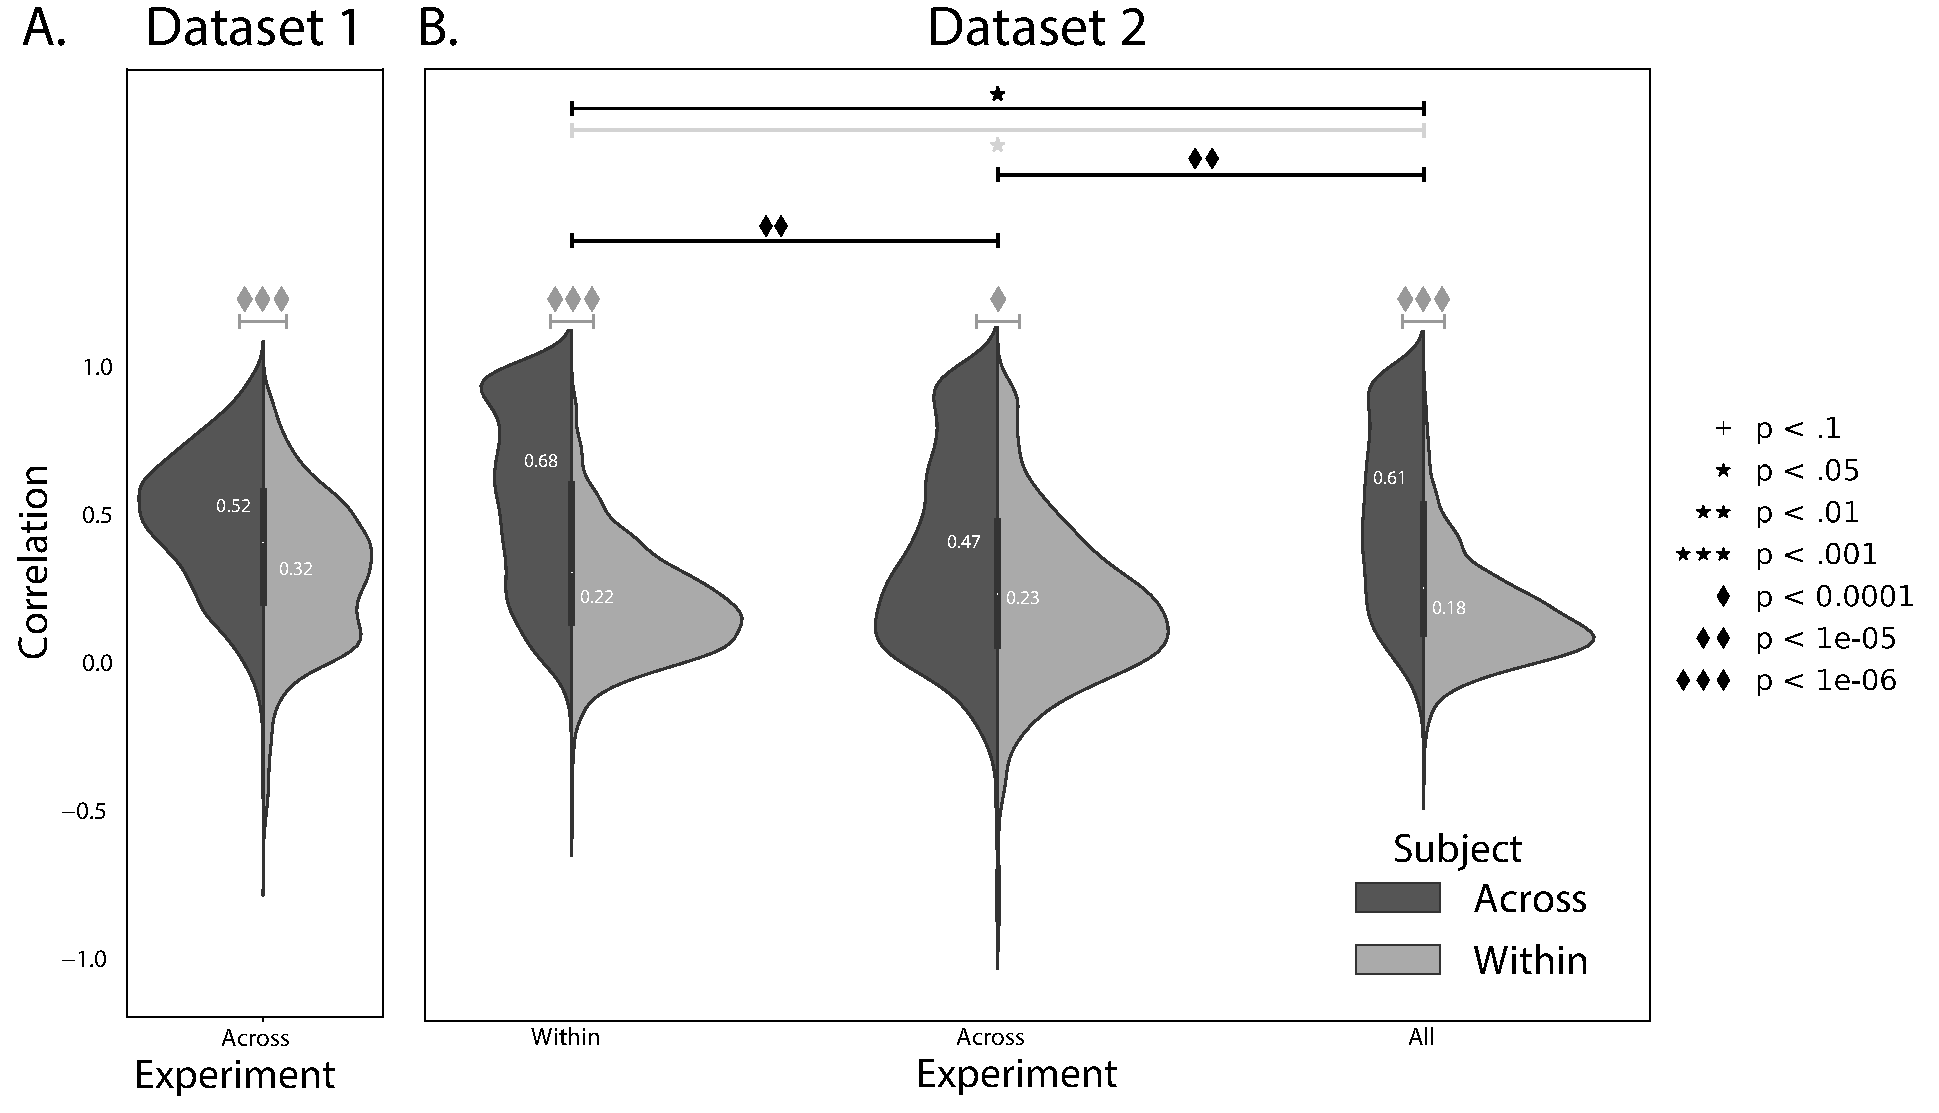
\includegraphics[width=0.75\textwidth]{figs/supplemental_1}
\caption{\small \textbf{Reconstruction quality for datasets 1 and 2.} \textbf{A. Distributions
      of correlation coefficients.}  Although patients in dataset 1 all participated in the same experiment, we did not limit our analyses to task specific data.  Instead we incorporated data from their entire recording session (sometimes up to 14 hours of data) and classify this as training our model on across experiment information. The split violin plot shows the distributions of reconstruction accuracy using models trained on data from all other patients (Across Subject, in black) and all other electrodes from the same patient (Within Subject, in gray). \textbf{B.  Distributions of correlation coefficients.} Since all patients participated in two experiments in dataset 2, we limit our analyses to task specific data.  The violin plots compare distributions of reconstruction accuracy using data from the same task (Within Experiment), the other task (Across Experiment), and from both tasks (All Experiment), using models trained on data from all other patients (Across Subject, in black) and all other electrodes from the same patient (Within Subject, in gray).}
\label{fig:supplemental_1}
\end{figure}


\begin{figure}[ptb]
\centering
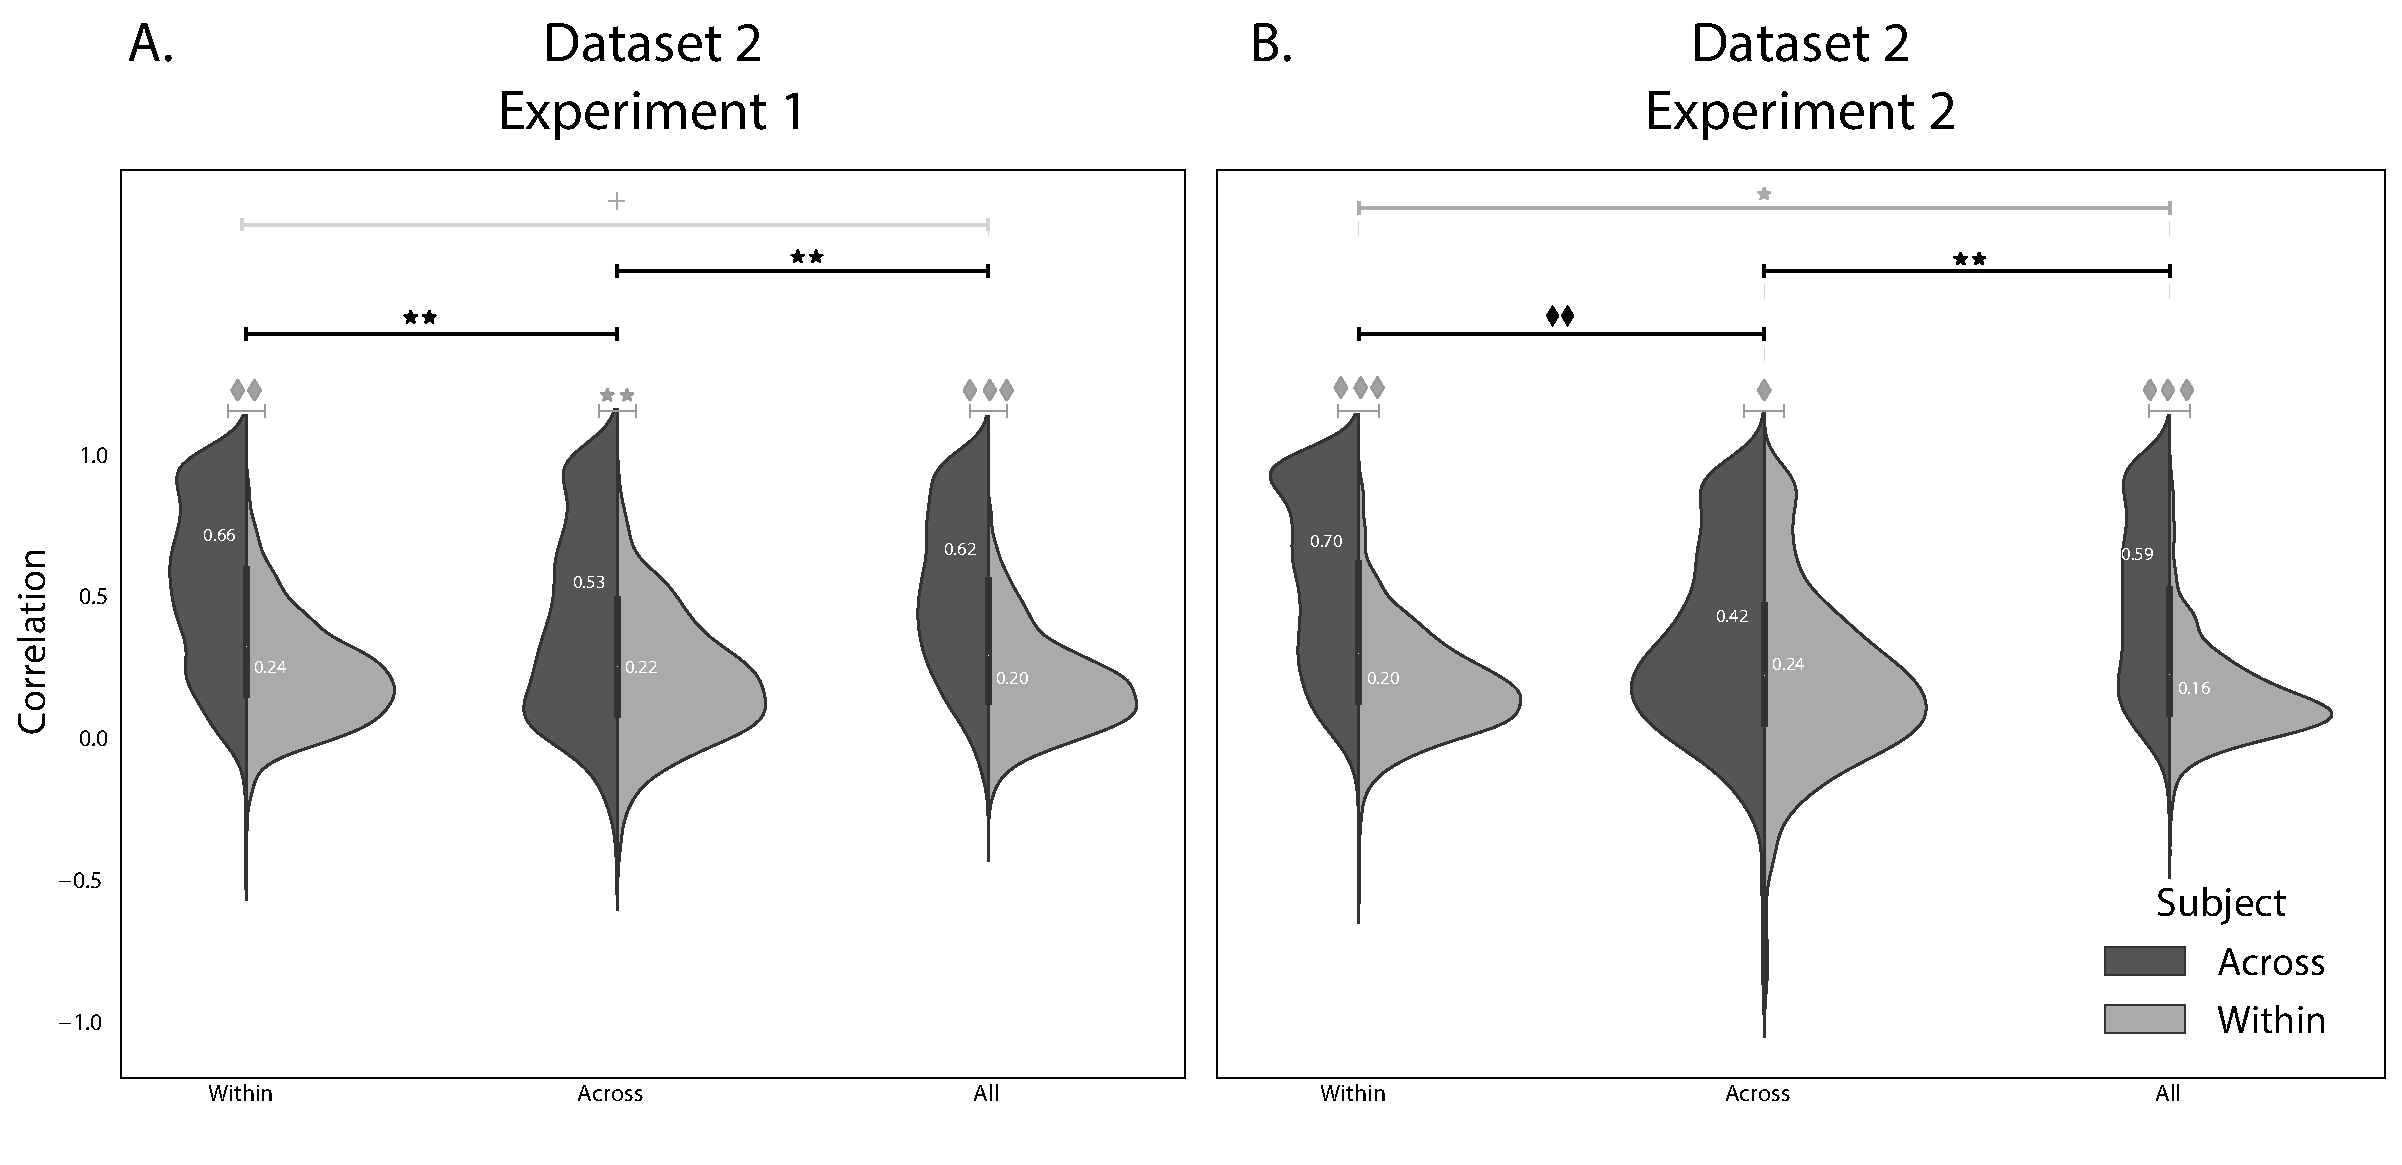
\includegraphics[width=\textwidth]{figs/supplemental_2}
\caption{\small \textbf{Reconstruction quality for experiments 1 and 2.} \textbf{A. Distributions
      of correlation coefficients.} For experiment 1, the split violin plots compare distributions of reconstruction accuracy using data from just experiment 1 (Within Experiment), just experiment 2 (Across Experiment), and from both experiments (All Experiment), using models trained on data from all other patients (Across Subject, in black) and all other electrodes from the same patient (Within Subject, in gray). \textbf{B.  Distributions
      of correlation coefficients.} For experiment 2, the split violin plots compare distributions of reconstruction accuracy using data from just experiment 2 (Within Experiment), just experiment 1 (Across Experiment), and from both experiments (All Experiment), using models trained on data from all other patients (Across Subject, in black) and all other electrodes from the same patient (Within Subject, in gray). }
\label{fig:supplemental_2}
\end{figure}

\begin{figure}[ptb]
\centering
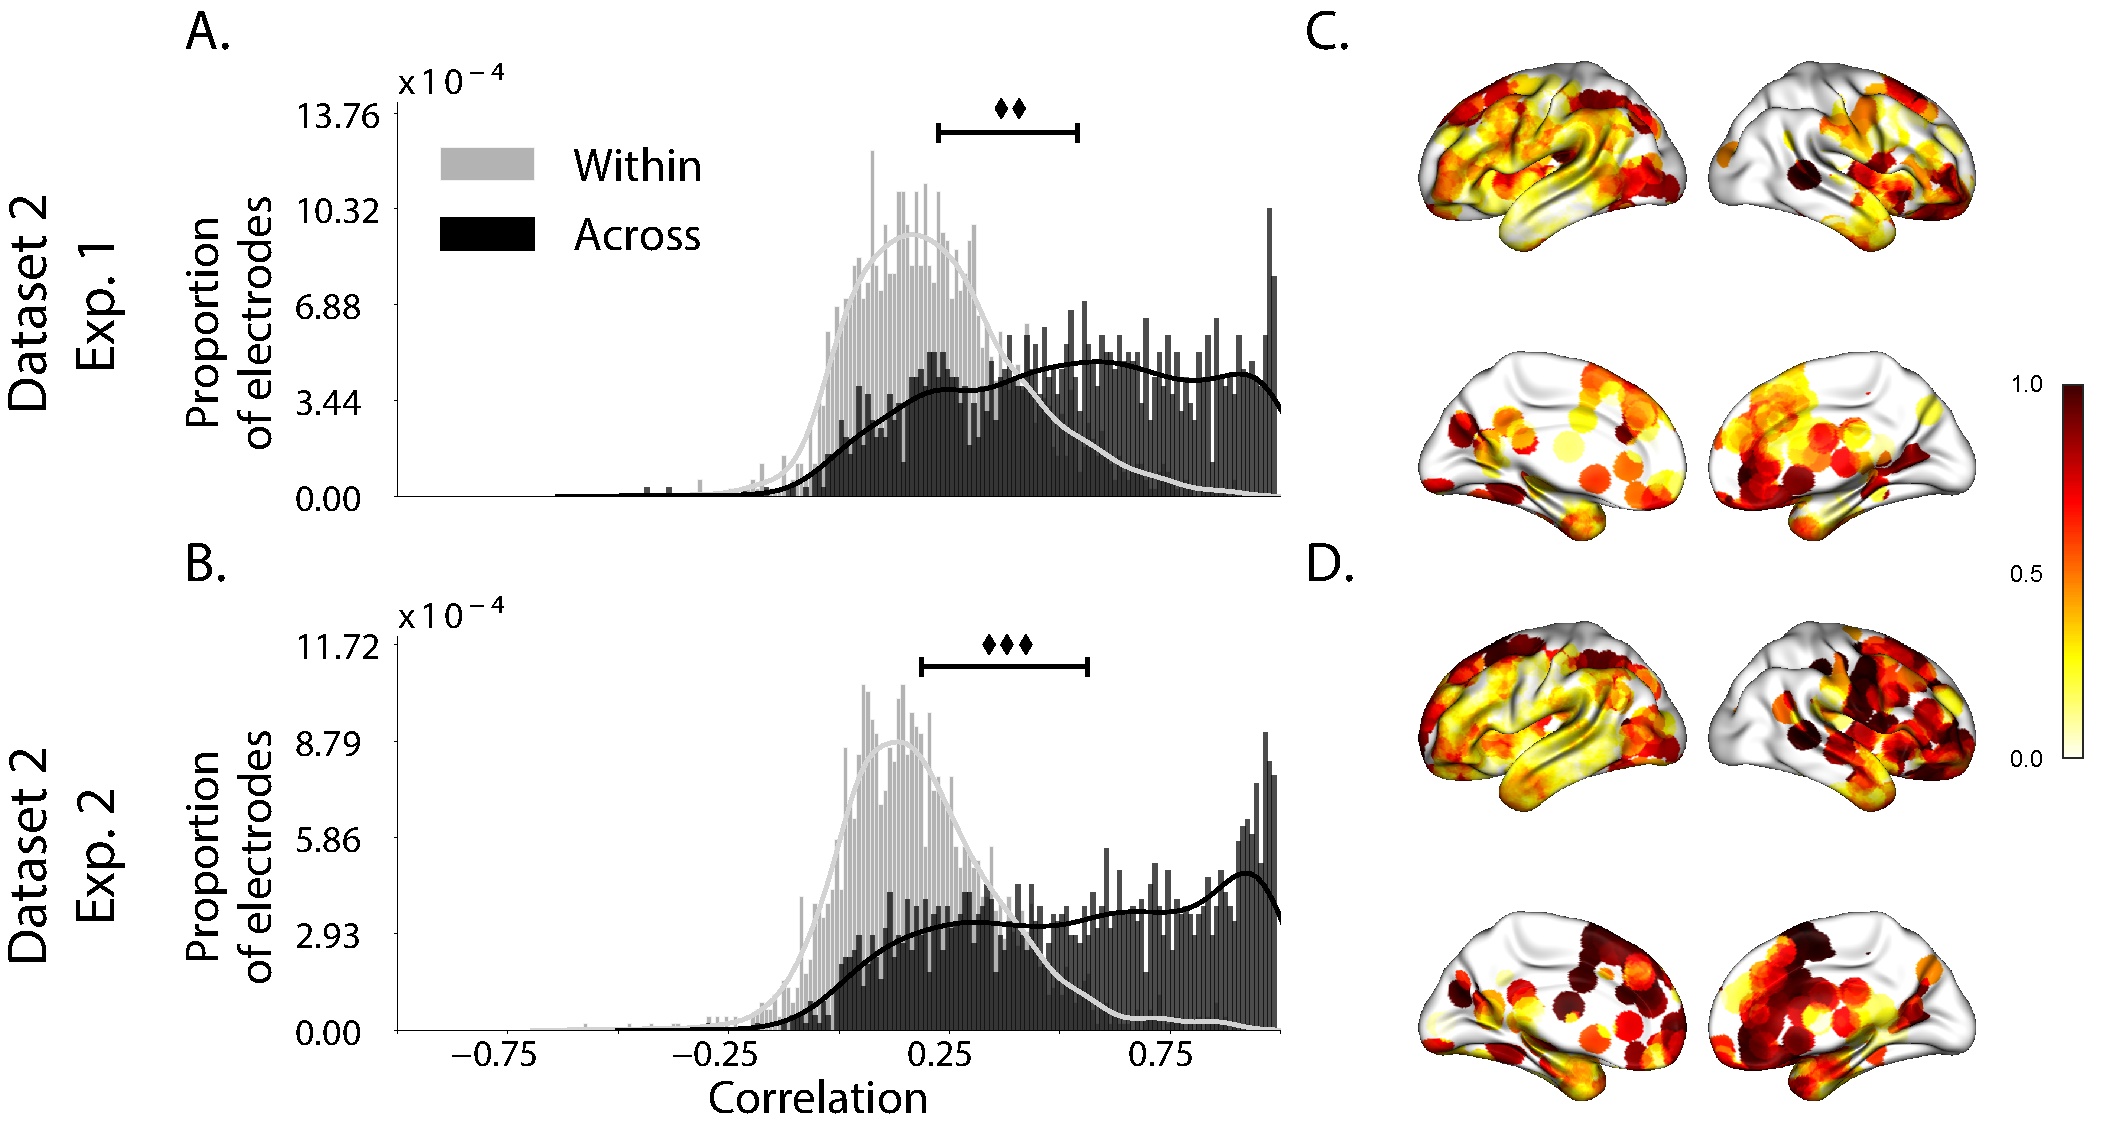
\includegraphics[width=\textwidth]{figs/supplemental_3}
\caption{\small \textbf{Reconstruction quality for each experiment.} \textbf{A. \& C.  Distributions
      of correlation coefficients.}  Across all electrodes from all
    patients in the labeled experiment from dataset 2, the panel displays the distribution of correlations between the observed and reconstructed LFP data using models trained on data from all other patients (Across, in black) and all other electrodes from the same patient (Within, in gray). 
    \textbf{B. \& D. Correlation maps.}  The glass brain maps display the
    average correlation between the observed LFP data and the across-subjects model reconstructed data by location, for each labeled experiment.}
\label{fig:supplemental_3}
\end{figure}


\begin{figure}[ptb]
\centering
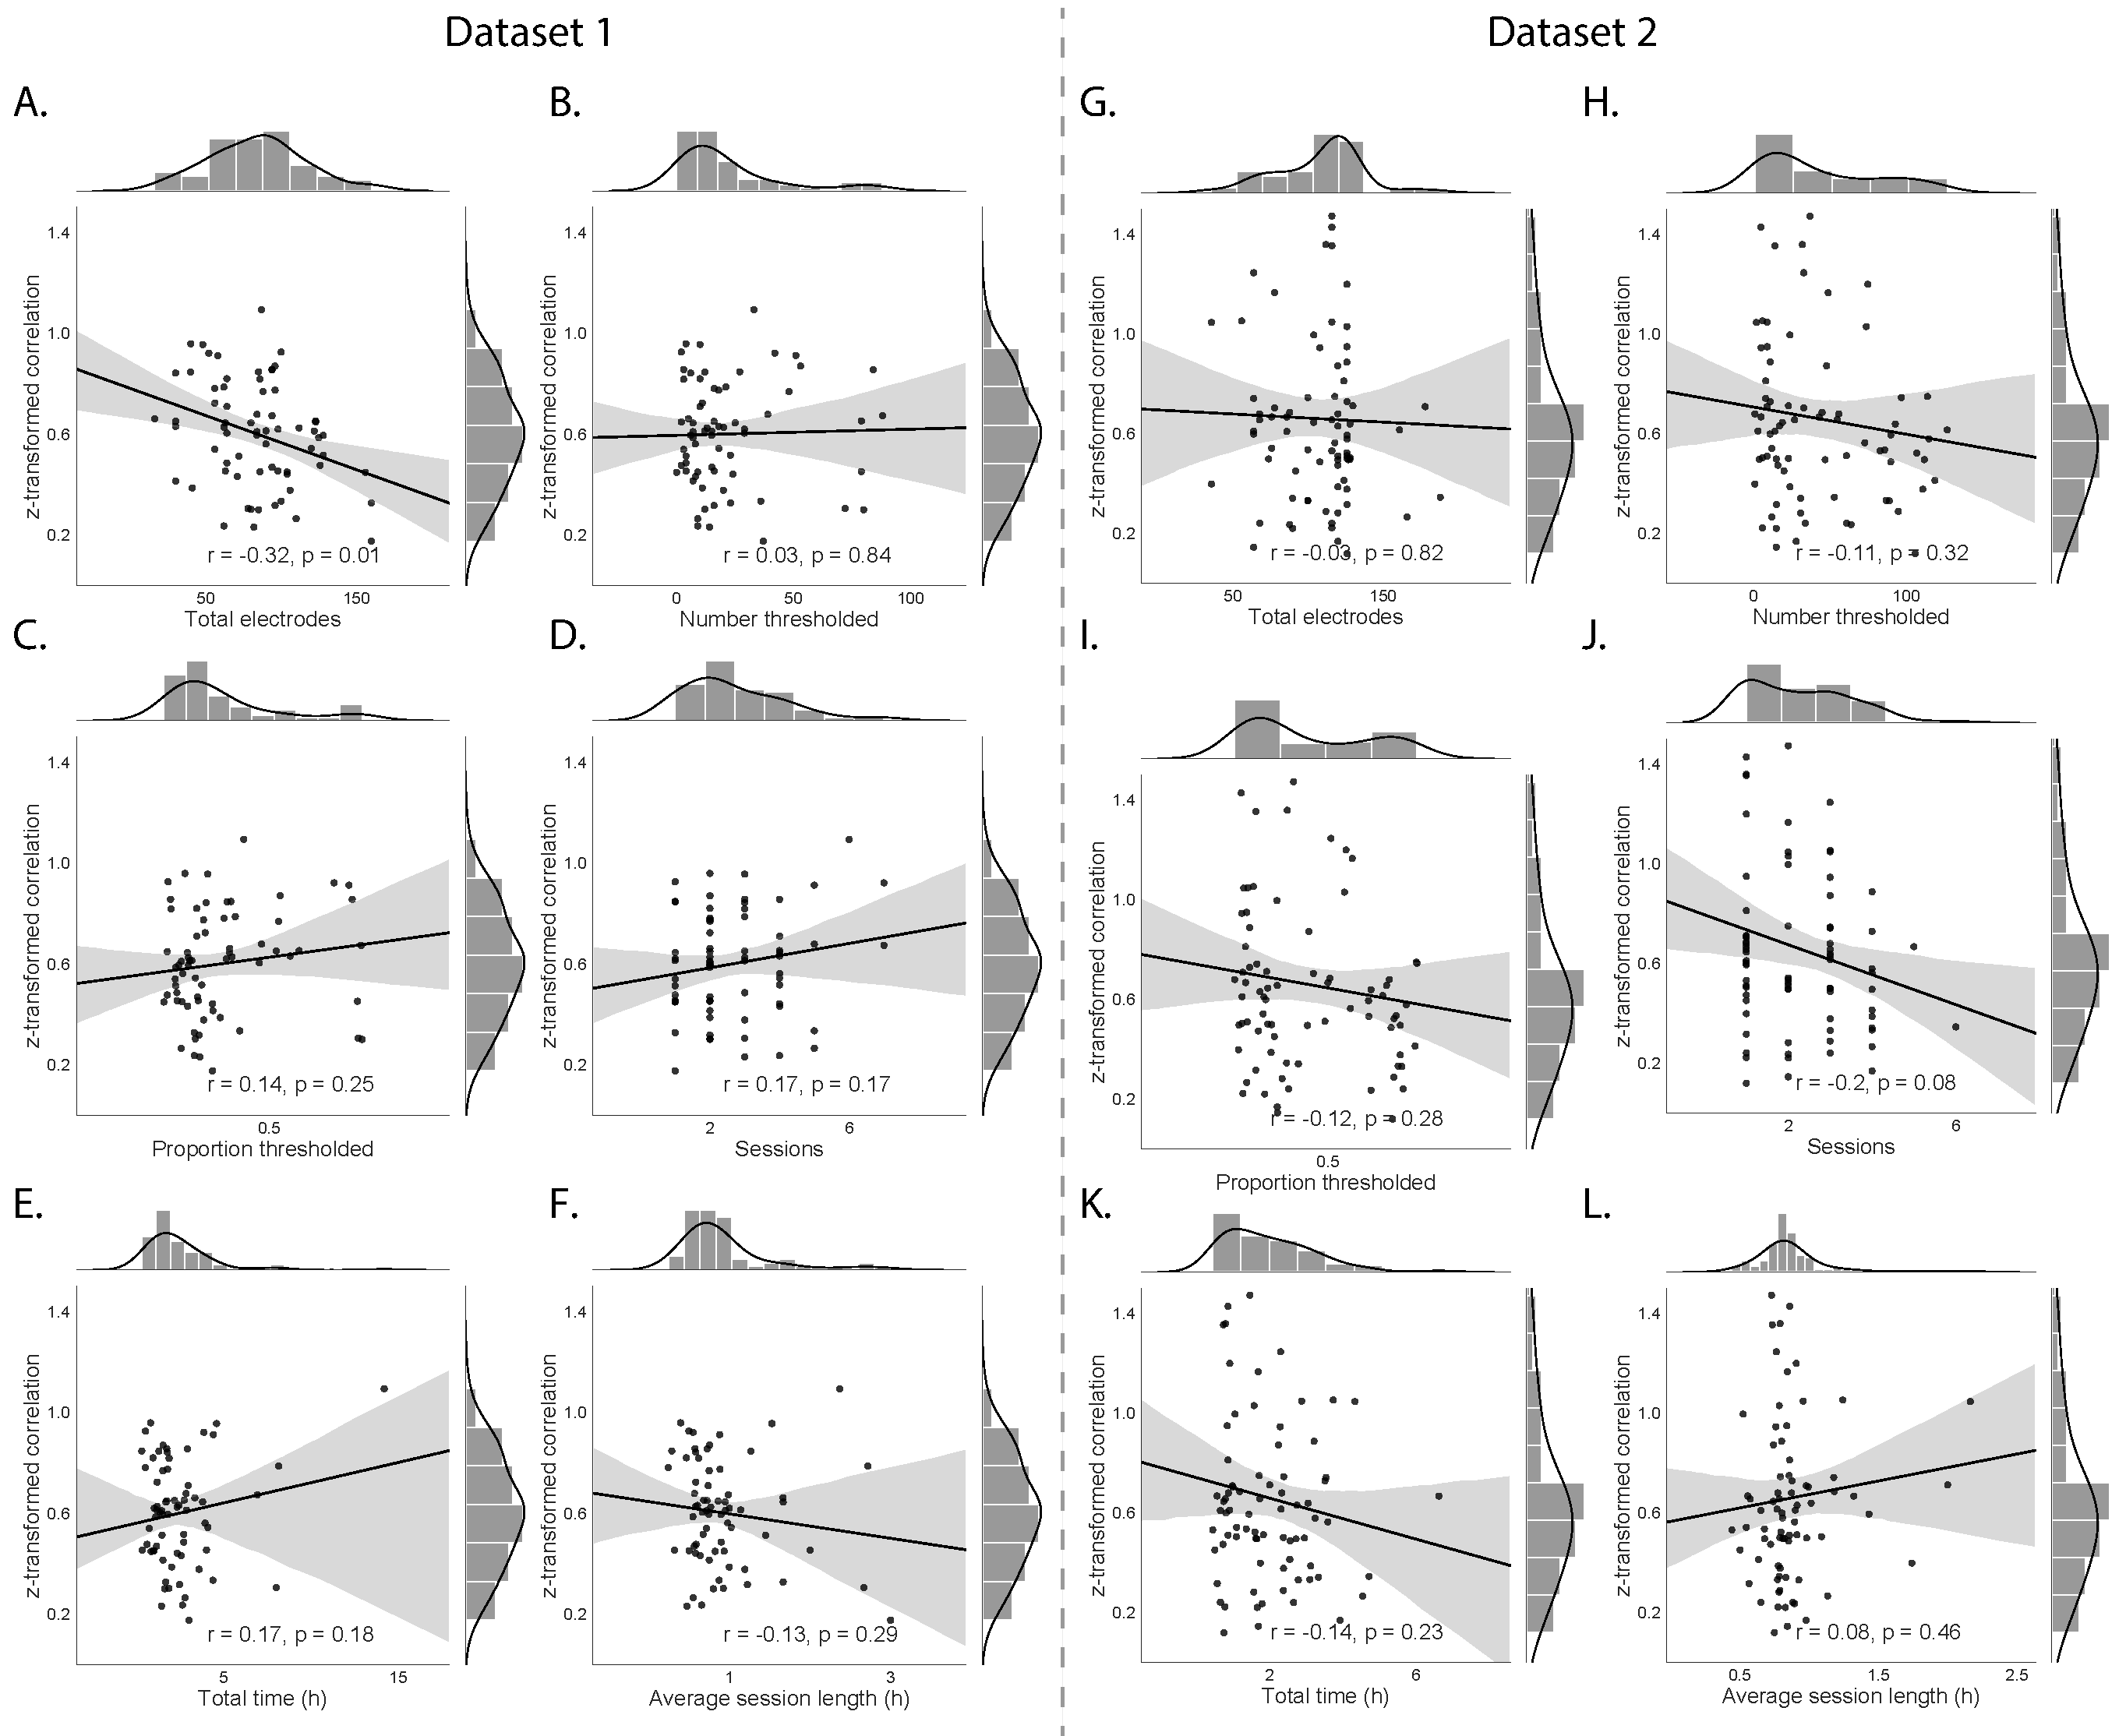
\includegraphics[width=\textwidth]{figs/supplemental_4}
\caption{\small \textbf{Reconstruction accuracy predicted by data
    features for each dataset.} \textbf{A.-F. \& G.-L.  Correspondence
    between average
    reconstruction accuracy
    and data feature for datasets 1 and 2.} The scatterplots display the z-transformed
  average patient correlation coefficient versus different features of
  the data (\textbf{A. \& G.} total electrodes, \textbf{B. \& H.}  proportion thresholded, \textbf{C. \& I.} total recording time,
  \textbf{D. \& J.}  number thresholded, \textbf{E. \& K.}  number of sessions, and \textbf{F. \& L.}  average session
  length). The one-dimensional histograms report the distribution of
  the z-transformed correlation coeffiencients and the associated data
feature.}
\label{fig:supplemental_4}
\end{figure}


\begin{figure}[ptb]
\centering
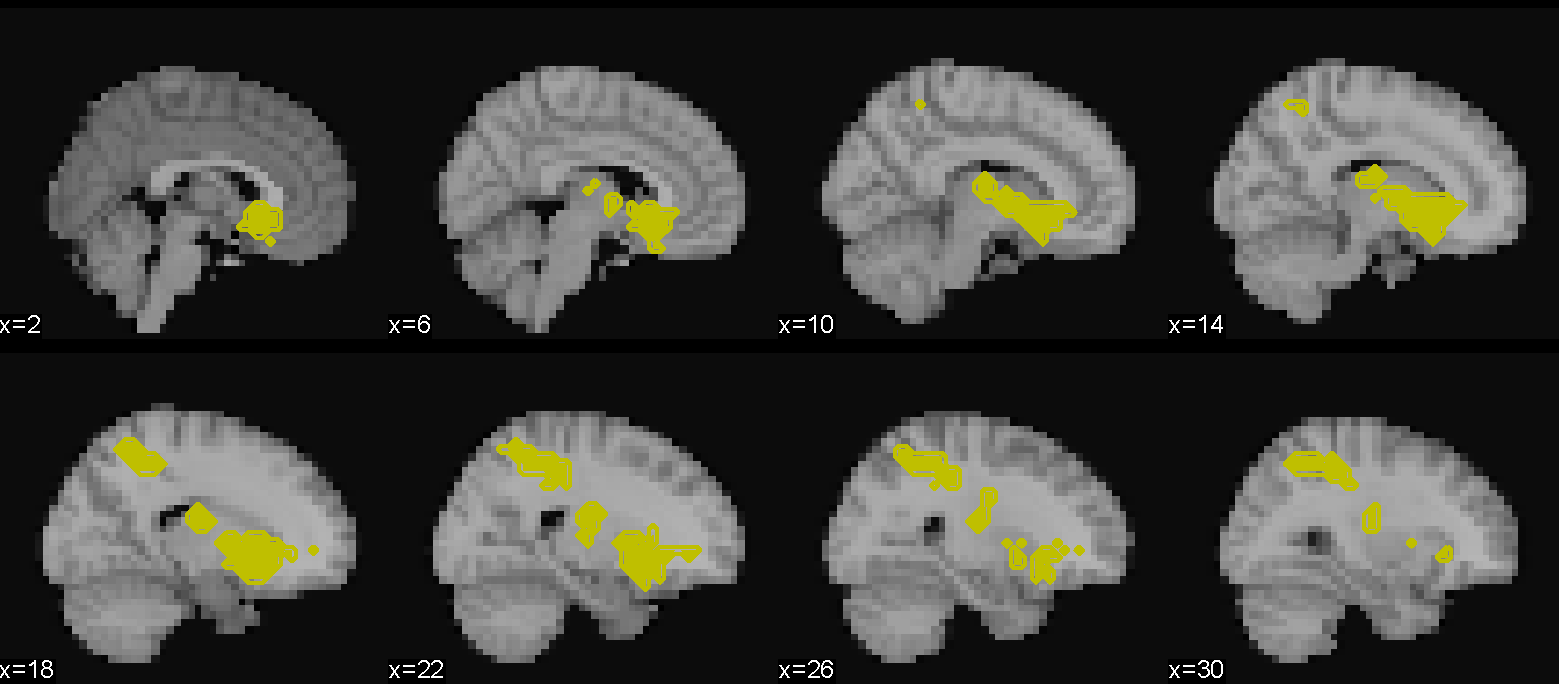
\includegraphics[width=\textwidth]{figs/supplemental_5}
\caption{\small \textbf{ Top 10\% most informative voxels.}
 Voxels in yellow indicate the intersections between
    the top 10\% most informative voxels in each brain map from Figure
    5, indicated by the white contours.}
\label{fig:supplemental_5}
\end{figure}


% \newpage
% \renewcommand{\refname}{Supplemental references}
% \bibliography{memlab}


\end{document}